% This is samplepaper.tex, a sample chapter demonstrating the
% LLNCS macro package for Springer Computer Science proceedings;
% Version 2.21 of 2022/01/12
%
\documentclass[runningheads]{llncs}
%
\usepackage[T1]{fontenc}
% T1 fonts will be used to generate the final print and online PDFs,
% so please use T1 fonts in your manuscript whenever possible.
% Other font encondings may result in incorrect characters.
%
\usepackage{graphicx}
\usepackage{amsmath}
% Used for displaying a sample figure. If possible, figure files should
% be included in EPS format.
%
% If you use the hyperref package, please uncomment the following two lines
% to display URLs in blue roman font according to Springer's eBook style:
%\usepackage{color}
%\renewcommand\UrlFont{\color{blue}\rmfamily}
%\urlstyle{rm}
%
\begin{document}
%
\title{Human-Computer Interaction approach with Empathic Conversational Agent and Computer Vision}
%
%\titlerunning{Abbreviated paper title}
% If the paper title is too long for the running head, you can set
% an abbreviated paper title here
%
\author{First Author\inst{1}\orcidID{0000-1111-2222-3333} \and
Second Author\inst{2,3}\orcidID{1111-2222-3333-4444} \and
Third Author\inst{3}\orcidID{2222--3333-4444-5555}}
%
\authorrunning{F. Author et al.}
% First names are abbreviated in the running head.
% If there are more than two authors, 'et al.' is used.
%
\institute{Princeton University, Princeton NJ 08544, USA \and
Springer Heidelberg, Tiergartenstr. 17, 69121 Heidelberg, Germany
\email{lncs@springer.com}\\
\url{http://www.springer.com/gp/computer-science/lncs} \and
ABC Institute, Rupert-Karls-University Heidelberg, Heidelberg, Germany\\
\email{\{abc,lncs\}@uni-heidelberg.de}}
%
\maketitle              % typeset the header of the contribution
%
\begin{abstract}
The abstract should briefly summarize the contents of the paper in
150--250 words.

\keywords{First keyword  \and Second keyword \and Another keyword.}
\end{abstract}
%
%
%

\section{Introduction}

Empathy, which entails comprehending and sharing others' emotions to forge emotional connections, is vital for human relationships. Similarly, in Human-Computer Interaction (HCI), empathy is crucial in ensuring more realistic, improved, convenient and meaningful interactions. However, the typical HCI, aimed at tailoring computer systems to meet the specific needs and preferences of individuals, still lacks the users' emotional state, therefore losing crucial information during these interactions \cite{jaiswal_facial_2020}.  Recent Artificial Intelligence (AI) techniques, such as Emotion Recognition (ER) and empathic Conversational Agents (CAs), when integrated with HCI allow for continuous understanding of the user's emotions throughout interactions and empathically providing responses, greatly contribute to an increase in the quality and deepness of interactions between humans and computers, improving the user's overall experience \cite{santos_approaches_2018}.

Artificial Intelligence (AI) encompasses various techniques and methodologies aimed at enabling machines to perform tasks that typically require human intelligence, whereas Deep Learning (DL) stands out as a specialized approach relying on Artificial Neural Networks (ANN) to process unstructured data (including images, voice, videos, and text, among others). ER, being a recent application of AI combined with DL, involves detecting human emotions through various modalities ranging from facial features, gestures, and poses, to speech and text captured through continuous interactions with the user \cite{alrowais_modified_2023}.  CAs consist of computer programs designed to simulate human-like conversation and engage in interactions with users through natural language using various techniques, including natural language processing (NLP), ML, and DL, to understand user input, interpret context, and generate appropriate responses.
 
Due to the immense potential of ER and CA, individually, and the numerous benefits provided when integrated with HCI, this study offers a comprehensive guide covering ER modalities and key design and functionality aspects of a CA, furthermore reviewing widely adopted datasets and methodologies. Lastly, proposing an innovative HCI approach to ensure more realistic and meaningful interactions by leveraging HCI in conjunction with ER techniques and an empathic CA.
 
The primary findings of this study can be summarized as follows:
\begin{itemize}
	\item Detailed guide on how DL impacts HCI nowadays;
	\item Performed a literature review regarding ER and CAs;
	\item Explored the main methods and datasets used for ER and CAs;
	\item Proposal of a taxonomy encompassing HCI, DL, CA, and ER;
	\item Proposal of an architecture of an HCI approach aided with ER, through Computer Vision (CV) and Sentiment Analysis (SA), and emphatic CA.
\end{itemize}

This research is organized into six sections. Section \ref{sec:background} presents the main concepts behind DL, ER, and CA. Section \ref{sec:datasets} details the most used datasets to train, validate, and evaluate ER and CA algorithms. Section \ref{sec:methods} introduces and discusses the core AI algorithms used nowadays to build ER systems and CAs, while Section \ref{sec:solution} presents the architecture, features, and characteristics of our proposed solution for HCI aided with ER and an empathic CA. Lastly, Section \ref{sec:conclusions}  introduces the challenges and directions for future work and the conclusions. 

\section{Background}
\label{sec:background}

The evolution of technology has led to an increased demand for advanced HCI. This is no longer confined to basic hardware-based communication but now encompasses more sophisticated techniques that are gradually becoming a part of everyday life. These include voice recognition, face recognition, and gesture recognition, which are essential for facilitating more natural and intuitive interactions between humans and computers \cite{Alrowais2023}. Furthermore, the ability of machines to perceive and interact with humans, whether in physical or virtual environments, needs an understanding of human motion. This understanding must account for physical constraints, such as muscle torque and gravity, as well as the intentions behind movements, making motion modeling a highly complex \cite{Martinez2017}.

Deep learning, a subset of machine learning, has been crucial in advancing the capabilities of HCI. By utilizing computational models with multiple processing layers, deep learning makes easier the learning of data representations at several levels of abstraction. This has significantly enhanced performance in domains like speech recognition, visual object recognition, object detection, and even fields like drug discovery and genomics. The focus of this paper will be on supervised learning, a predominant form of deep learning. Supervised learning involves training a system with a labeled dataset, where the system learns to map inputs to outputs based on example input-output pairs. During training, the system iteratively adjusts its parameters to minimize the difference between its outputs and the desired outputs. This process involves a high number of adjustable parameters, or weights, which define the system's input-output function \cite{Lecun2015} \cite{Mahony2020}.

The implementation of deep learning in supervised learning models follows a structured process. This encompasses phases like data collection, where the importance of data quality cannot be overstated, data preprocessing to enhance data quality, training the model, optimization based on validation, and testing \cite{Schmidhuber2015}. In recent years, Facial Emotion Recognition (FER) systems have exemplified the efficacy of Artificial Neural Networks (ANNs) over traditional machine learning methods. ANNs have demonstrated superior performance in detecting and recognizing emotions in a subject-independent manner, analyzing training data from various individuals. This approach has opened new opportunities in fields like healthcare, security, business, education, and manufacturing \cite{Giannopoulos2018} \cite{Cirneanu2023} \cite{Zhao2015}.

In the context of computer vision, neural networks have been particularly successful in image classification tasks, including face identification and facial emotion recognition. These technologies are not only used in surveillance systems but also in medical diagnostics and user-interactive applications. Different neural network architectures have been employed to meet the specific requirements of these tasks, including the use of pre-trained networks for classification, feature extraction, and transfer learning. Transfer learning, in particular, involves adjusting and reusing layers of a neural network trained on one dataset to work with a new dataset, demonstrating the versatility and adaptability of neural networks in various applications \cite{Cirneanu2023} \cite{Zhao2015}.

Deep learning processes rely on data collection and processing, notably for image-based models. The quality of data is crucial for a model's learning efficacy. To mitigate issues such as overfitting, which refers to the phenomenon where a network learns a function with very high variance to perfectly model the training data \cite{Shorten2019}, data augmentation can be used. This technique generates new training samples by applying transformations like rotation and scaling. It's essential for diversifying the training dataset, particularly in cases of low amounts of data \cite{Khalifa2022}.

The evolution of deep learning has been marked by a shift from hand-engineered features to trainable multilayer networks, a concept realized through the implementation of backpropagation. This method allows the calculation of gradients in multilayer structures by working backward from the output. Convolutional Neural Networks (CNNs) architecture, shown in Figure \ref{fig:cnnarchitecture}, are an excellent example of this approach, they are structured with convolutional and pooling layers. These networks process multi-array data, like images, using local connections and shared weights. The convolutional layers consist of units organized in feature maps connected to local patches in previous layers, highlighting the principle of location invariance in data like images that fit when detecting emotions through computer vision \cite{Lecun2015}.

\begin{figure}[htb]
\centering
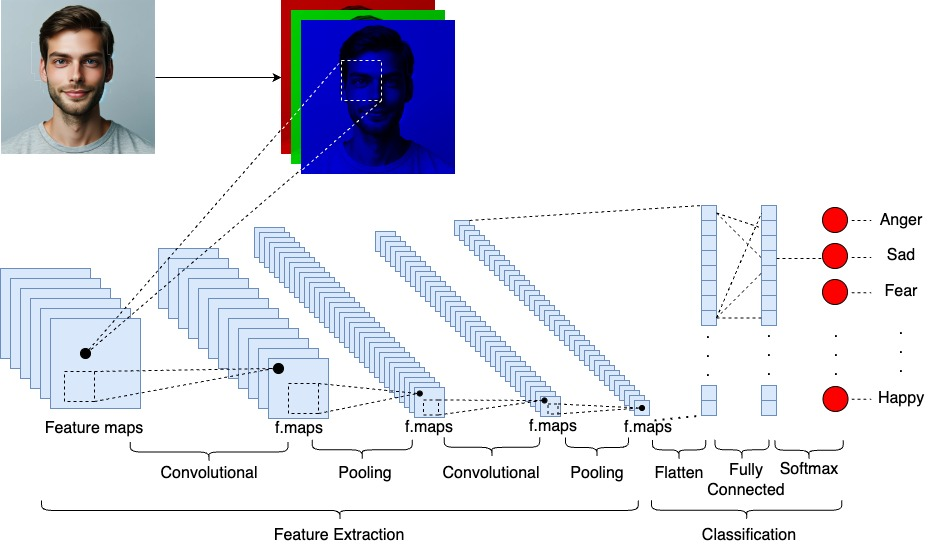
\includegraphics[width=0.97\linewidth]{CNNArchitecture.jpg}
\caption{An illustrative diagram of a CNN for emotion detection. The process begins with an input image of a smiling person and progresses through successive convolution and pooling layers for feature extraction. After flattening the feature maps, a fully connected network follows, leading to a final classification layer that categorizes the detected emotions into anger, sadness, fear, and happiness.}
\label{fig:cnnarchitecture}
\end{figure}

In CNN architecture, convolutional layers extract key features through their feature maps, while pooling layers further refine them by reducing their spatial size. This process improves the computational efficiency, and also increases the robustness of the features, a relevant aspect in the context of computer vision. Following this, the flattened layer transforms the two-dimensional feature maps into a one-dimensional vector, preparing them for the classification stage. This stage primarily involves fully connected layers, which interpret the extracted features and make decisions. The last layer typically employs a softmax function, shown in equation \ref{eq:sofmax}, converting the output into probabilities for each class. In this context, transfer learning emerges as a significant strategy, allowing the transfer of knowledge from one model to another, particularly beneficial when training data is limited. It involves using pre-trained models on large datasets and adapting them to specific tasks, significantly reducing the need for extensive training data and computational resources \cite{Khan2020}.

\begin{equation}
\text{softmax}(z_i) = \frac{e^{z_i}}{\sum_{k=1}^{K} e^{z_k}} \quad \text{for} \, i = 1, 2, ..., K
\label{eq:sofmax}
\end{equation}

% ER with CV (Face, Pose, Text, Speech). Landmarks.

% CA (Embodied, Interaction, Domain, Goal)

\section{Datasets}
\label{sec:datasets}

% Introduce the main datasets used.

\section{Methods}
\label{sec:methods}

% Introduce the main methods used.

\section{Proposed solution}
\label{sec:solution}

% description of characteristics
% prototype ???

\section{Future work and conclusions}
\label{sec:conclusions}

\begin{credits}
\subsubsection{\ackname} A bold run-in heading in small font size at the end of the paper is
used for general acknowledgments, for example: This study was funded
by X (grant number Y).

\subsubsection{\discintname}
It is now necessary to declare any competing interests or to specifically
state that the authors have no competing interests. Please place the
statement with a bold run-in heading in small font size beneath the
(optional) acknowledgments\footnote{If EquinOCS, our proceedings submission
system, is used, then the disclaimer can be provided directly in the system.},
for example: The authors have no competing interests to declare that are
relevant to the content of this article. Or: Author A has received research
grants from Company W. Author B has received a speaker honorarium from
Company X and owns stock in Company Y. Author C is a member of committee Z.
\end{credits}
%
% ---- Bibliography ----
%
% BibTeX users should specify bibliography style 'splncs04'.
% References will then be sorted and formatted in the correct style.
%
\bibliographystyle{splncs04}
\bibliography{bibliography}
%
\end{document}
